\chapter{FLARE: Prototype System Design and Demonstration}

\section{Overview}

\textbf{FLARE} is the prototype system built as the primary applied deliverable of
this Honours project. It translates the theoretical LE-PSI protocol into a complete,
working sanctions screening web application, directly addressing the research question:
\textit{``Can post-quantum Laconic PSI be deployed in a real-world financial
compliance workflow?''}

FLARE implements a two-party architecture where a Financial Institution (client)
screens its customer database against a Sanctions Authority's watchlist --- without
either party exposing their raw data to the other. The prototype is fully functional
and was demonstrated running live, with end-to-end screening executed in real time.

The name FLARE reflects the system's purpose: a rapid, visible signal raised when a
customer match is detected against a sanctions list --- analogous to a flare used to
alert in high-stakes situations.

% ─────────────────────────────────────────────────────────────────────────────
\section{System Architecture}

FLARE simulates two geographically separated parties using four independent processes:

\begin{table}[H]
\centering
\caption{FLARE deployment components}
\label{tab:flare-arch}
\begin{tabular}{@{}lllll@{}}
\toprule
\textbf{Party} & \textbf{Process} & \textbf{Port} & \textbf{Database} & \textbf{Role} \\
\midrule
Financial Inst. & Next.js UI   & 3000 & ---      & Client dashboard \\
Financial Inst. & Go API       & 8080 & SQLite   & Customer data + PSI client \\
Sanctions Auth. & Next.js UI   & 3001 & ---      & Authority dashboard \\
Sanctions Auth. & Go API       & 8081 & PostgreSQL & Sanctions list + PSI server \\
\bottomrule
\end{tabular}
\end{table}

The two parties communicate exclusively over HTTPS with encrypted LE-PSI ciphertexts.
The sanctions authority learns nothing about which customers the bank is screening;
the bank learns nothing about non-matching entries in the sanctions list. Only matched
customer hashes cross the network --- no plaintext customer data is ever transmitted
between parties.

\subsection{Technology Stack}

\begin{itemize}
  \item \textbf{Backend}: Go 1.24, Chi HTTP router, JWT authentication with Role-Based
        Access Control (RBAC), Bcrypt password hashing, WebSocket for real-time job
        progress updates.
  \item \textbf{Frontend}: Next.js 16 (App Router), TypeScript 5, Tailwind CSS v4,
        shadcn/ui component library. A single codebase renders as either Client or
        Authority mode via the environment variable \texttt{NEXT\_PUBLIC\_APP\_MODE}.
  \item \textbf{Cryptography}: LE-PSI library (this project) via \texttt{psiadapter}
        module; Lattigo v3 for Ring-LWE primitives.
  \item \textbf{Databases}: PostgreSQL (Sanctions Authority, persistent list storage);
        SQLite (Financial Institution, local customer store).
\end{itemize}

\subsection{Data Normalisation Pipeline}

A critical engineering challenge in applying PSI to real-world identity data is ensuring
that the same real-world entity is hashed identically on both sides, despite variations
in data entry format. FLARE applies a five-step normalisation pipeline before hashing:

\begin{enumerate}
  \item \textbf{Lowercase and trim}: Remove leading/trailing whitespace and convert to lowercase.
  \item \textbf{ISO date format}: Normalise any date format to \texttt{YYYY-MM-DD}.
  \item \textbf{Country normalisation}: Map any country name or code to ISO-3166 alpha-2.
  \item \textbf{Concatenation}: Combine fields as \texttt{name|dob|country}.
  \item \textbf{SHA-256 $\to$ uint64}: Hash the concatenated string and truncate to a
        64-bit integer for LE-PSI input.
\end{enumerate}

\textbf{Example:} ``John Doe'', ``15 March 1985'', ``United States'' $\to$
\texttt{john doe|1985-03-15|us} $\to$ \texttt{0x7a3f9c2e1b8d4567}.

This pipeline ensures deterministic, format-independent identity matching without
transmitting any plaintext fields across party boundaries.

% ─────────────────────────────────────────────────────────────────────────────
\section{Prototype Walkthrough}

The following subsections present each screen of the running prototype with
annotations describing the observed behaviour and its connection to the underlying
LE-PSI protocol.

\subsection{Dashboard --- Operational Overview}

\begin{figure}[H]
\centering
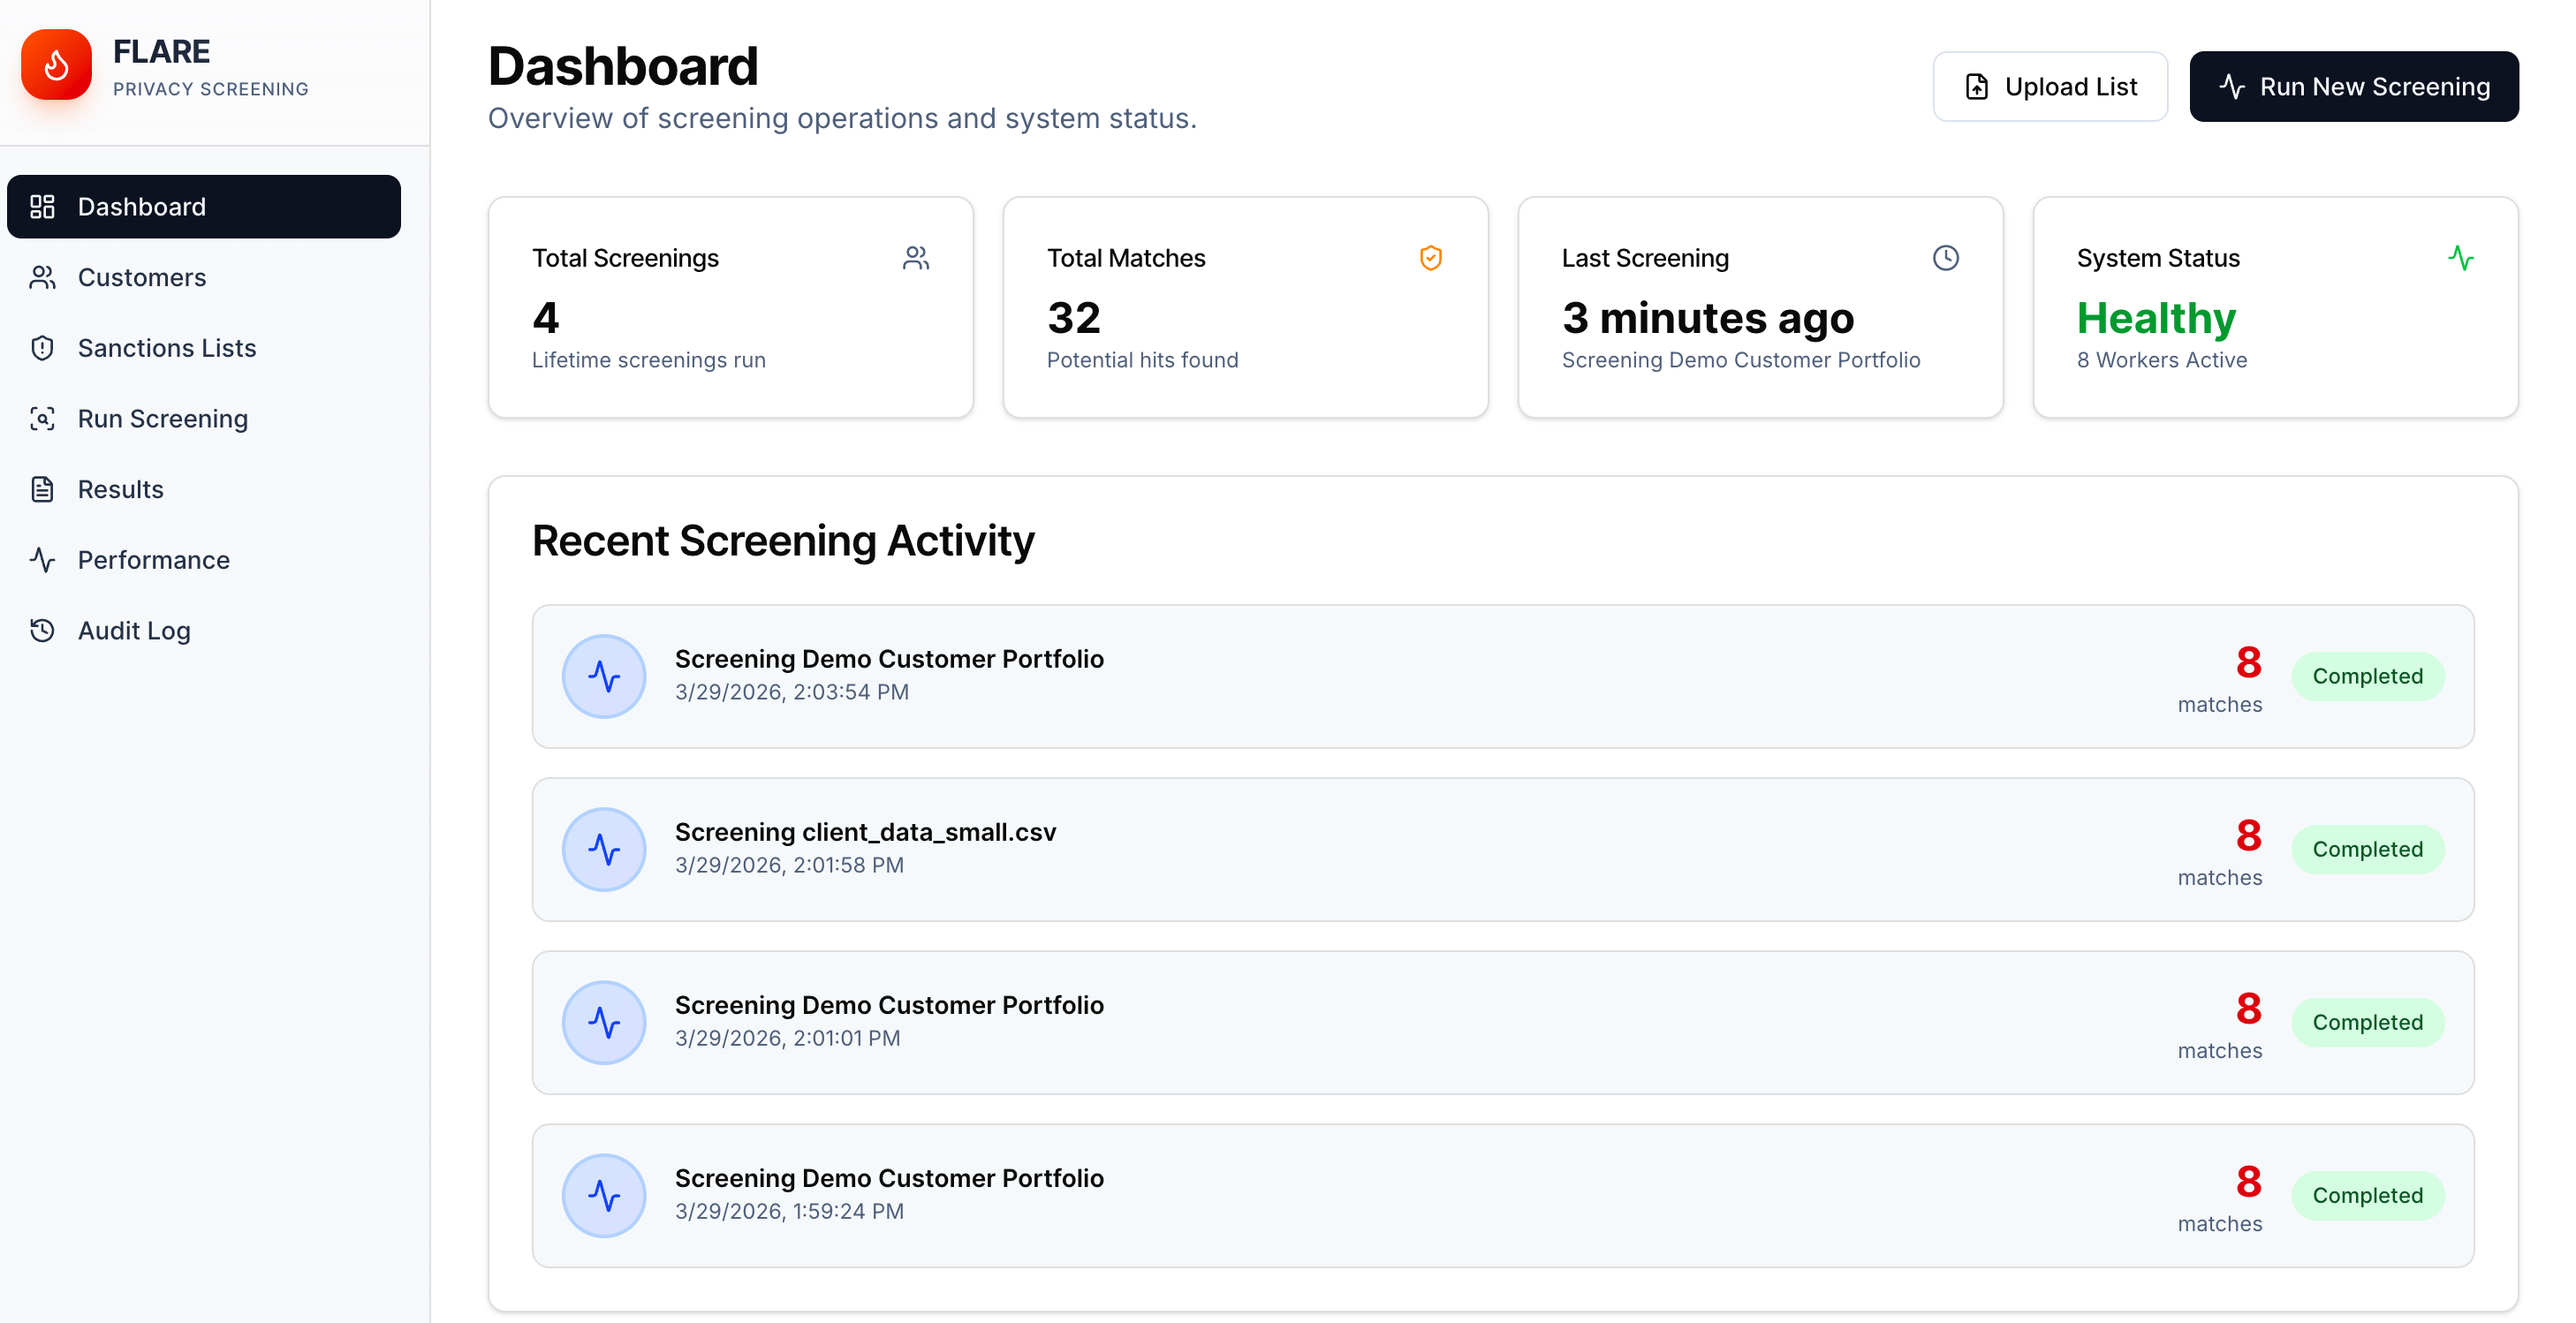
\includegraphics[width=0.95\textwidth]{prototype/dashboard.png}
\caption{FLARE Dashboard (Client/Bank side). Shows 4 completed screenings,
         32 total potential matches, and system status: Healthy with 8 active
         worker goroutines. Each row shows a screening job with its timestamp
         and match count. The ``Run New Screening'' and ``Upload List'' buttons
         initiate the two primary user workflows.}
\label{fig:proto-dashboard}
\end{figure}

The dashboard provides the Financial Institution's analyst with a real-time
operational view of all screening jobs. The \textit{System Status: Healthy} indicator
confirms the backend is connected and the LE-PSI worker pool is active. Each completed
screening shows a timestamp and match count. Consistent match counts across repeated
runs confirm that the LE-PSI cryptographic matching is deterministic --- a necessary
correctness property.

The dashboard initiates two primary workflows: uploading a customer list and running
a new screening job against the sanctions authority.

\subsection{Customer List Management}

\begin{figure}[H]
\centering
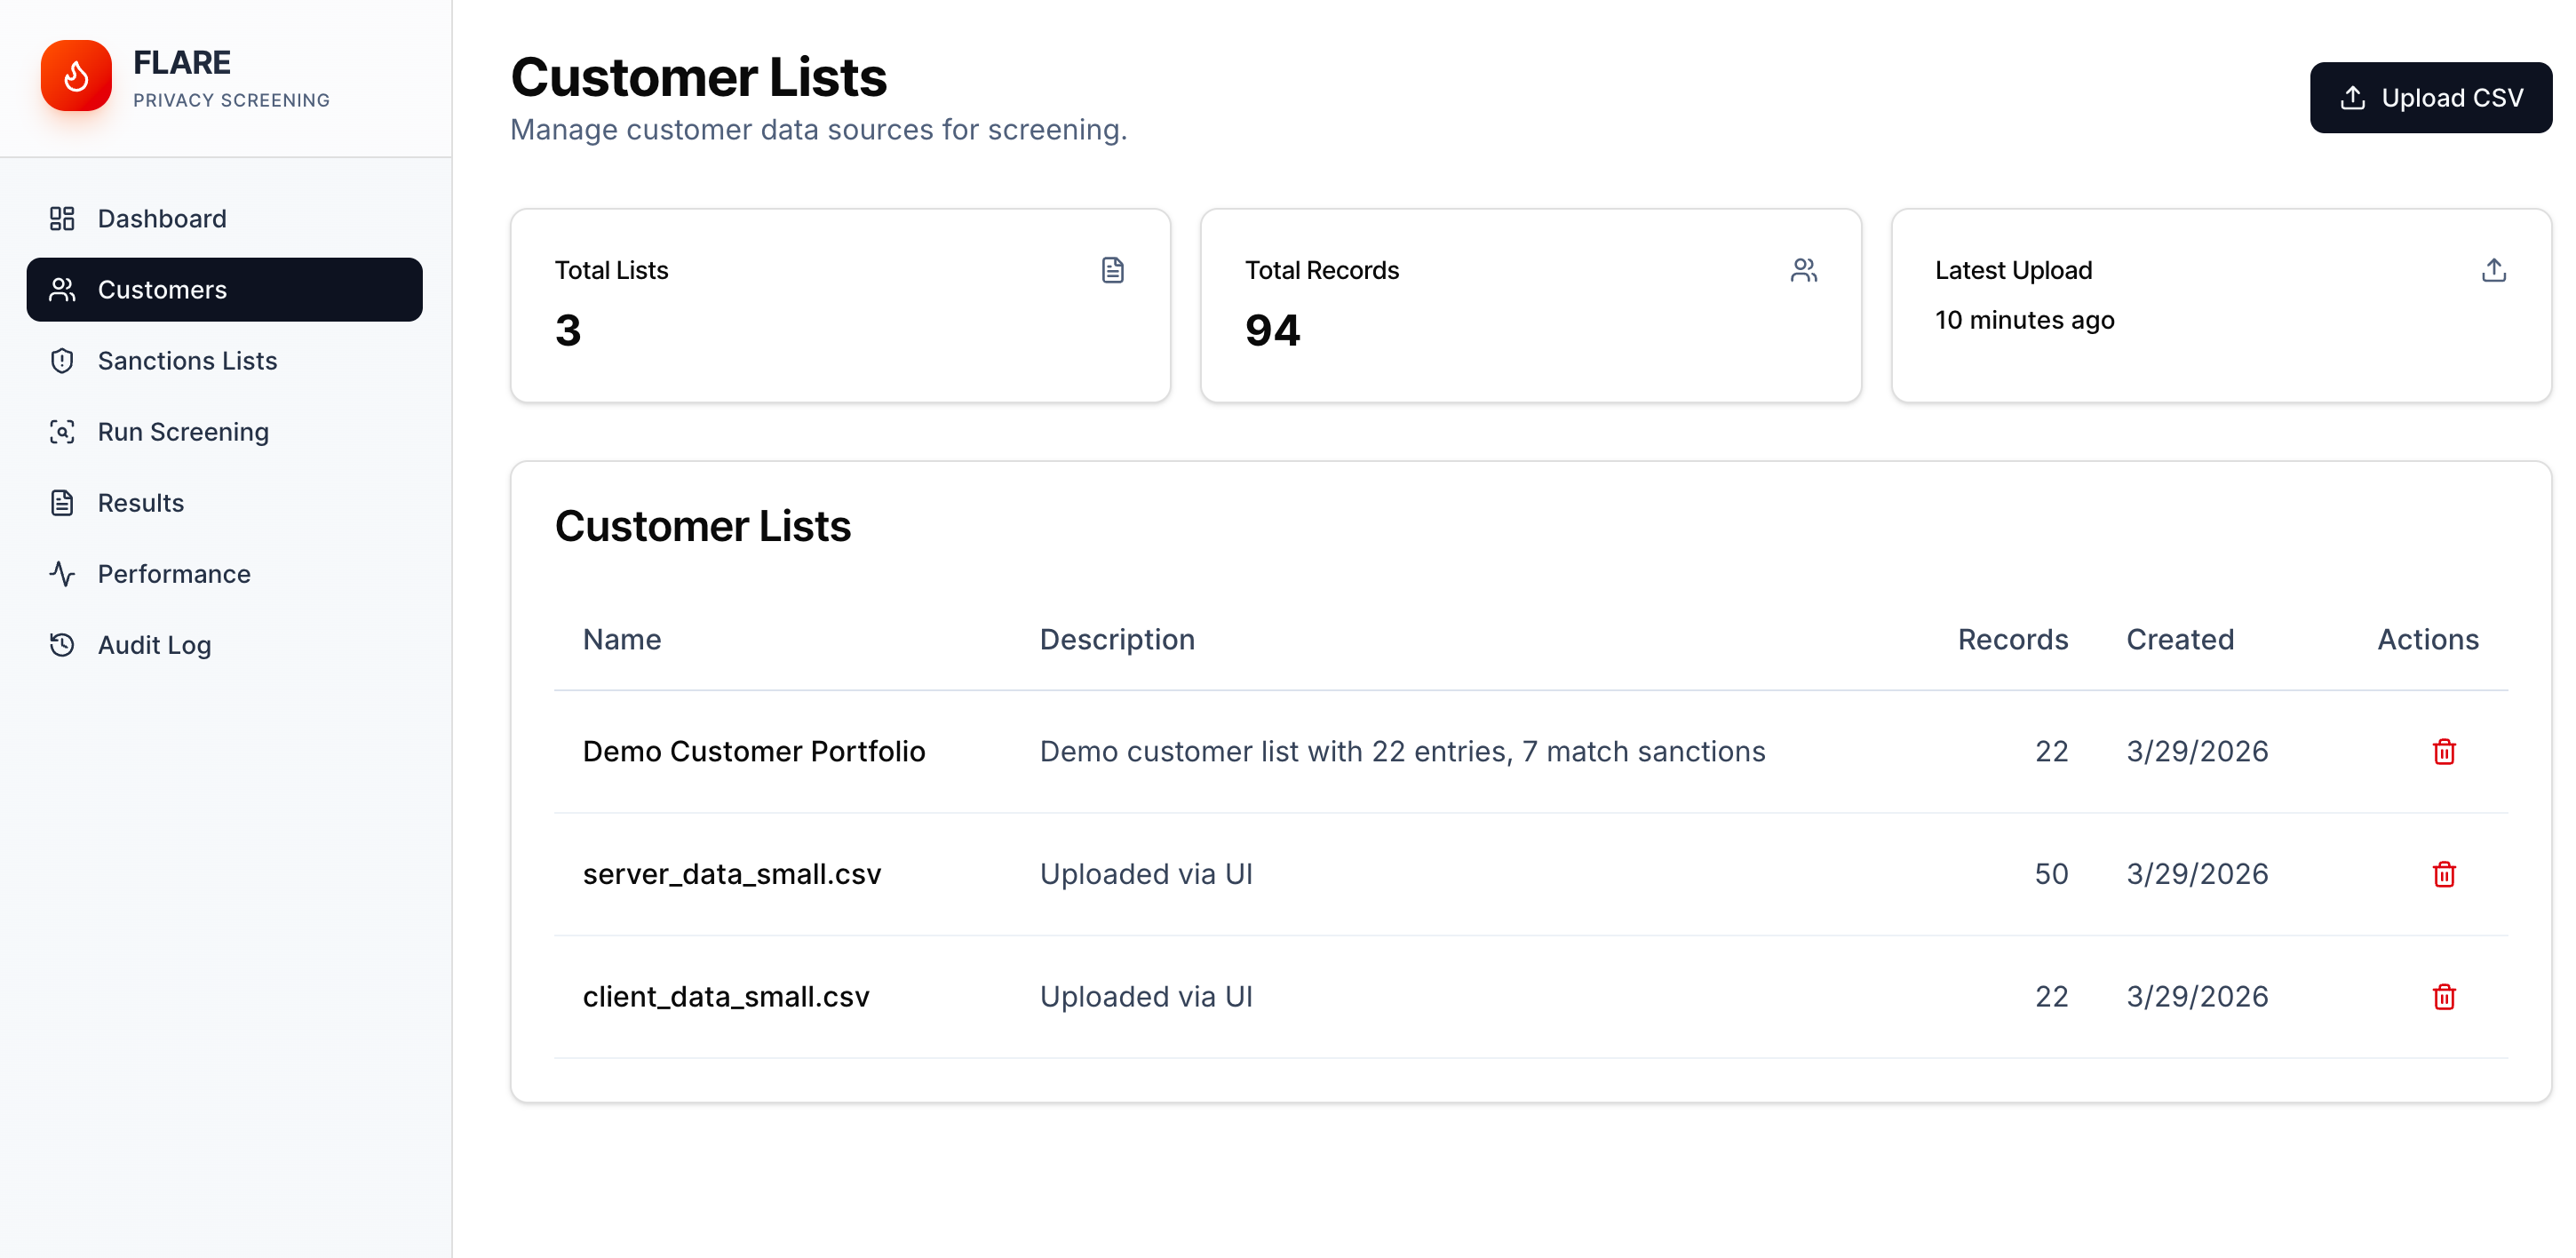
\includegraphics[width=0.95\textwidth]{prototype/customer_list.png}
\caption{Customer Lists page. The bank has uploaded 3 customer datasets
         totalling 94 records. The ``Demo Customer Portfolio'' (22 records)
         is the primary test set, known to contain 7 records that appear in
         the sanctions list.}
\label{fig:proto-customers}
\end{figure}

The Financial Institution uploads customer data as CSV files. FLARE stores these
locally in SQLite and applies the normalisation pipeline automatically on upload.
At no point does raw customer data leave the bank's own infrastructure in plaintext
--- the data remains on-premises until it is encrypted into Ring-LWE ciphertexts
for transmission.

\subsection{Sanctions List Management}

\begin{figure}[H]
\centering
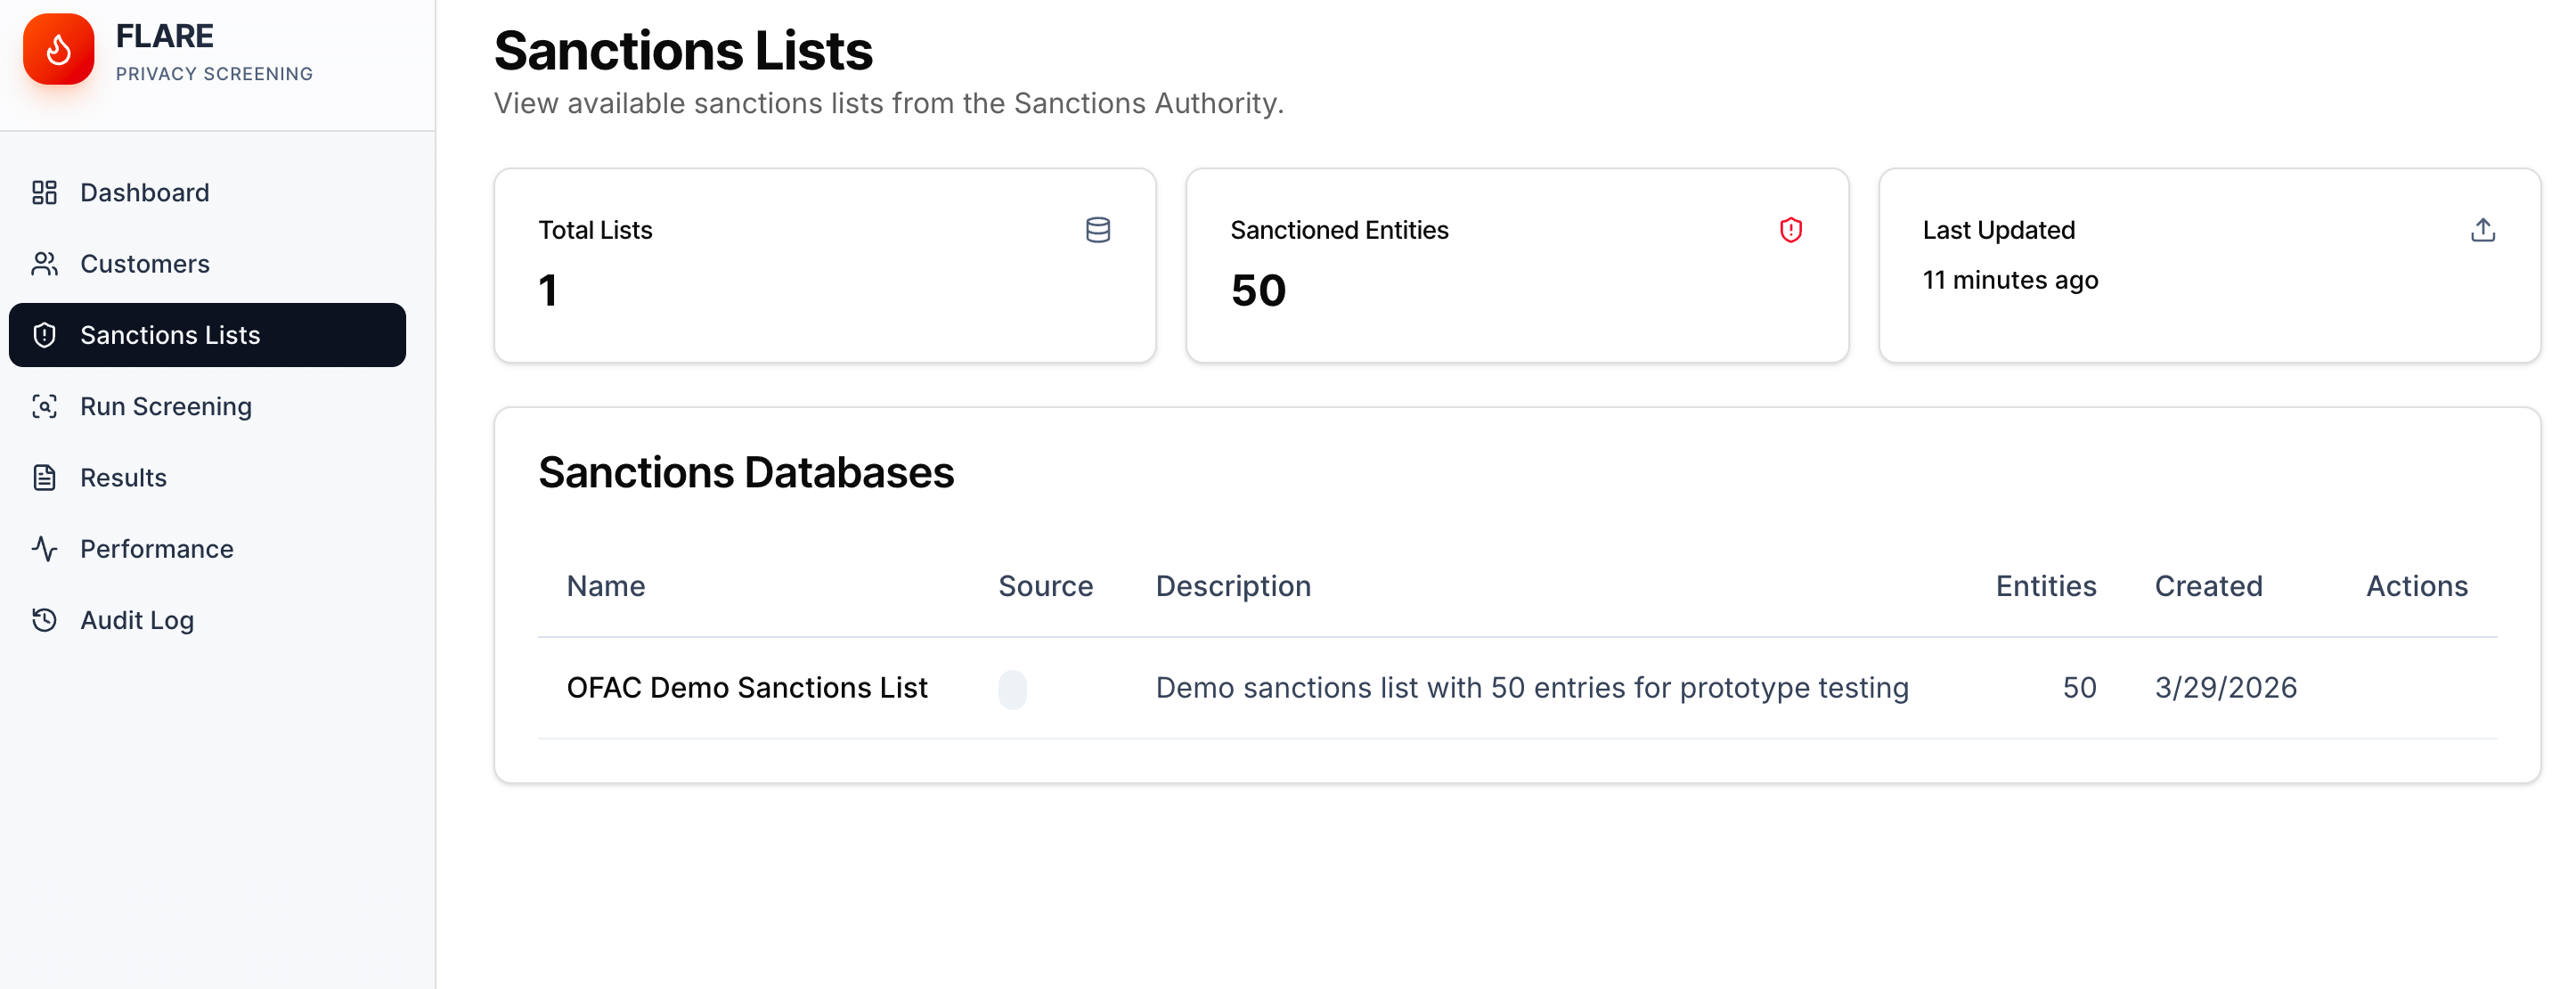
\includegraphics[width=0.95\textwidth]{prototype/sansaction_list.png}
\caption{Sanctions Lists page (Authority side). The OFAC Demo Sanctions List
         contains 50 sanctioned entities across terrorism financing, cyber
         crime, corruption, UN Security Council, and money laundering programs.
         The authority pre-computes LE-PSI public parameters against this list
         once, then reuses them for all future screening requests.}
\label{fig:proto-sanctions}
\end{figure}

The Sanctions Authority maintains its watchlist in PostgreSQL and pre-computes
the Merkle tree and LE public parameters offline. This offline server initialisation
--- the $O(m \log m)$ key generation and tree construction phase --- is the
computationally expensive one-time setup cost. It is repeated only when the
sanctions list changes, meaning the per-screening amortised cost of the server's
first message is effectively zero.

\subsection{Run Screening --- Privacy-Preserving Execution}

\begin{figure}[H]
\centering
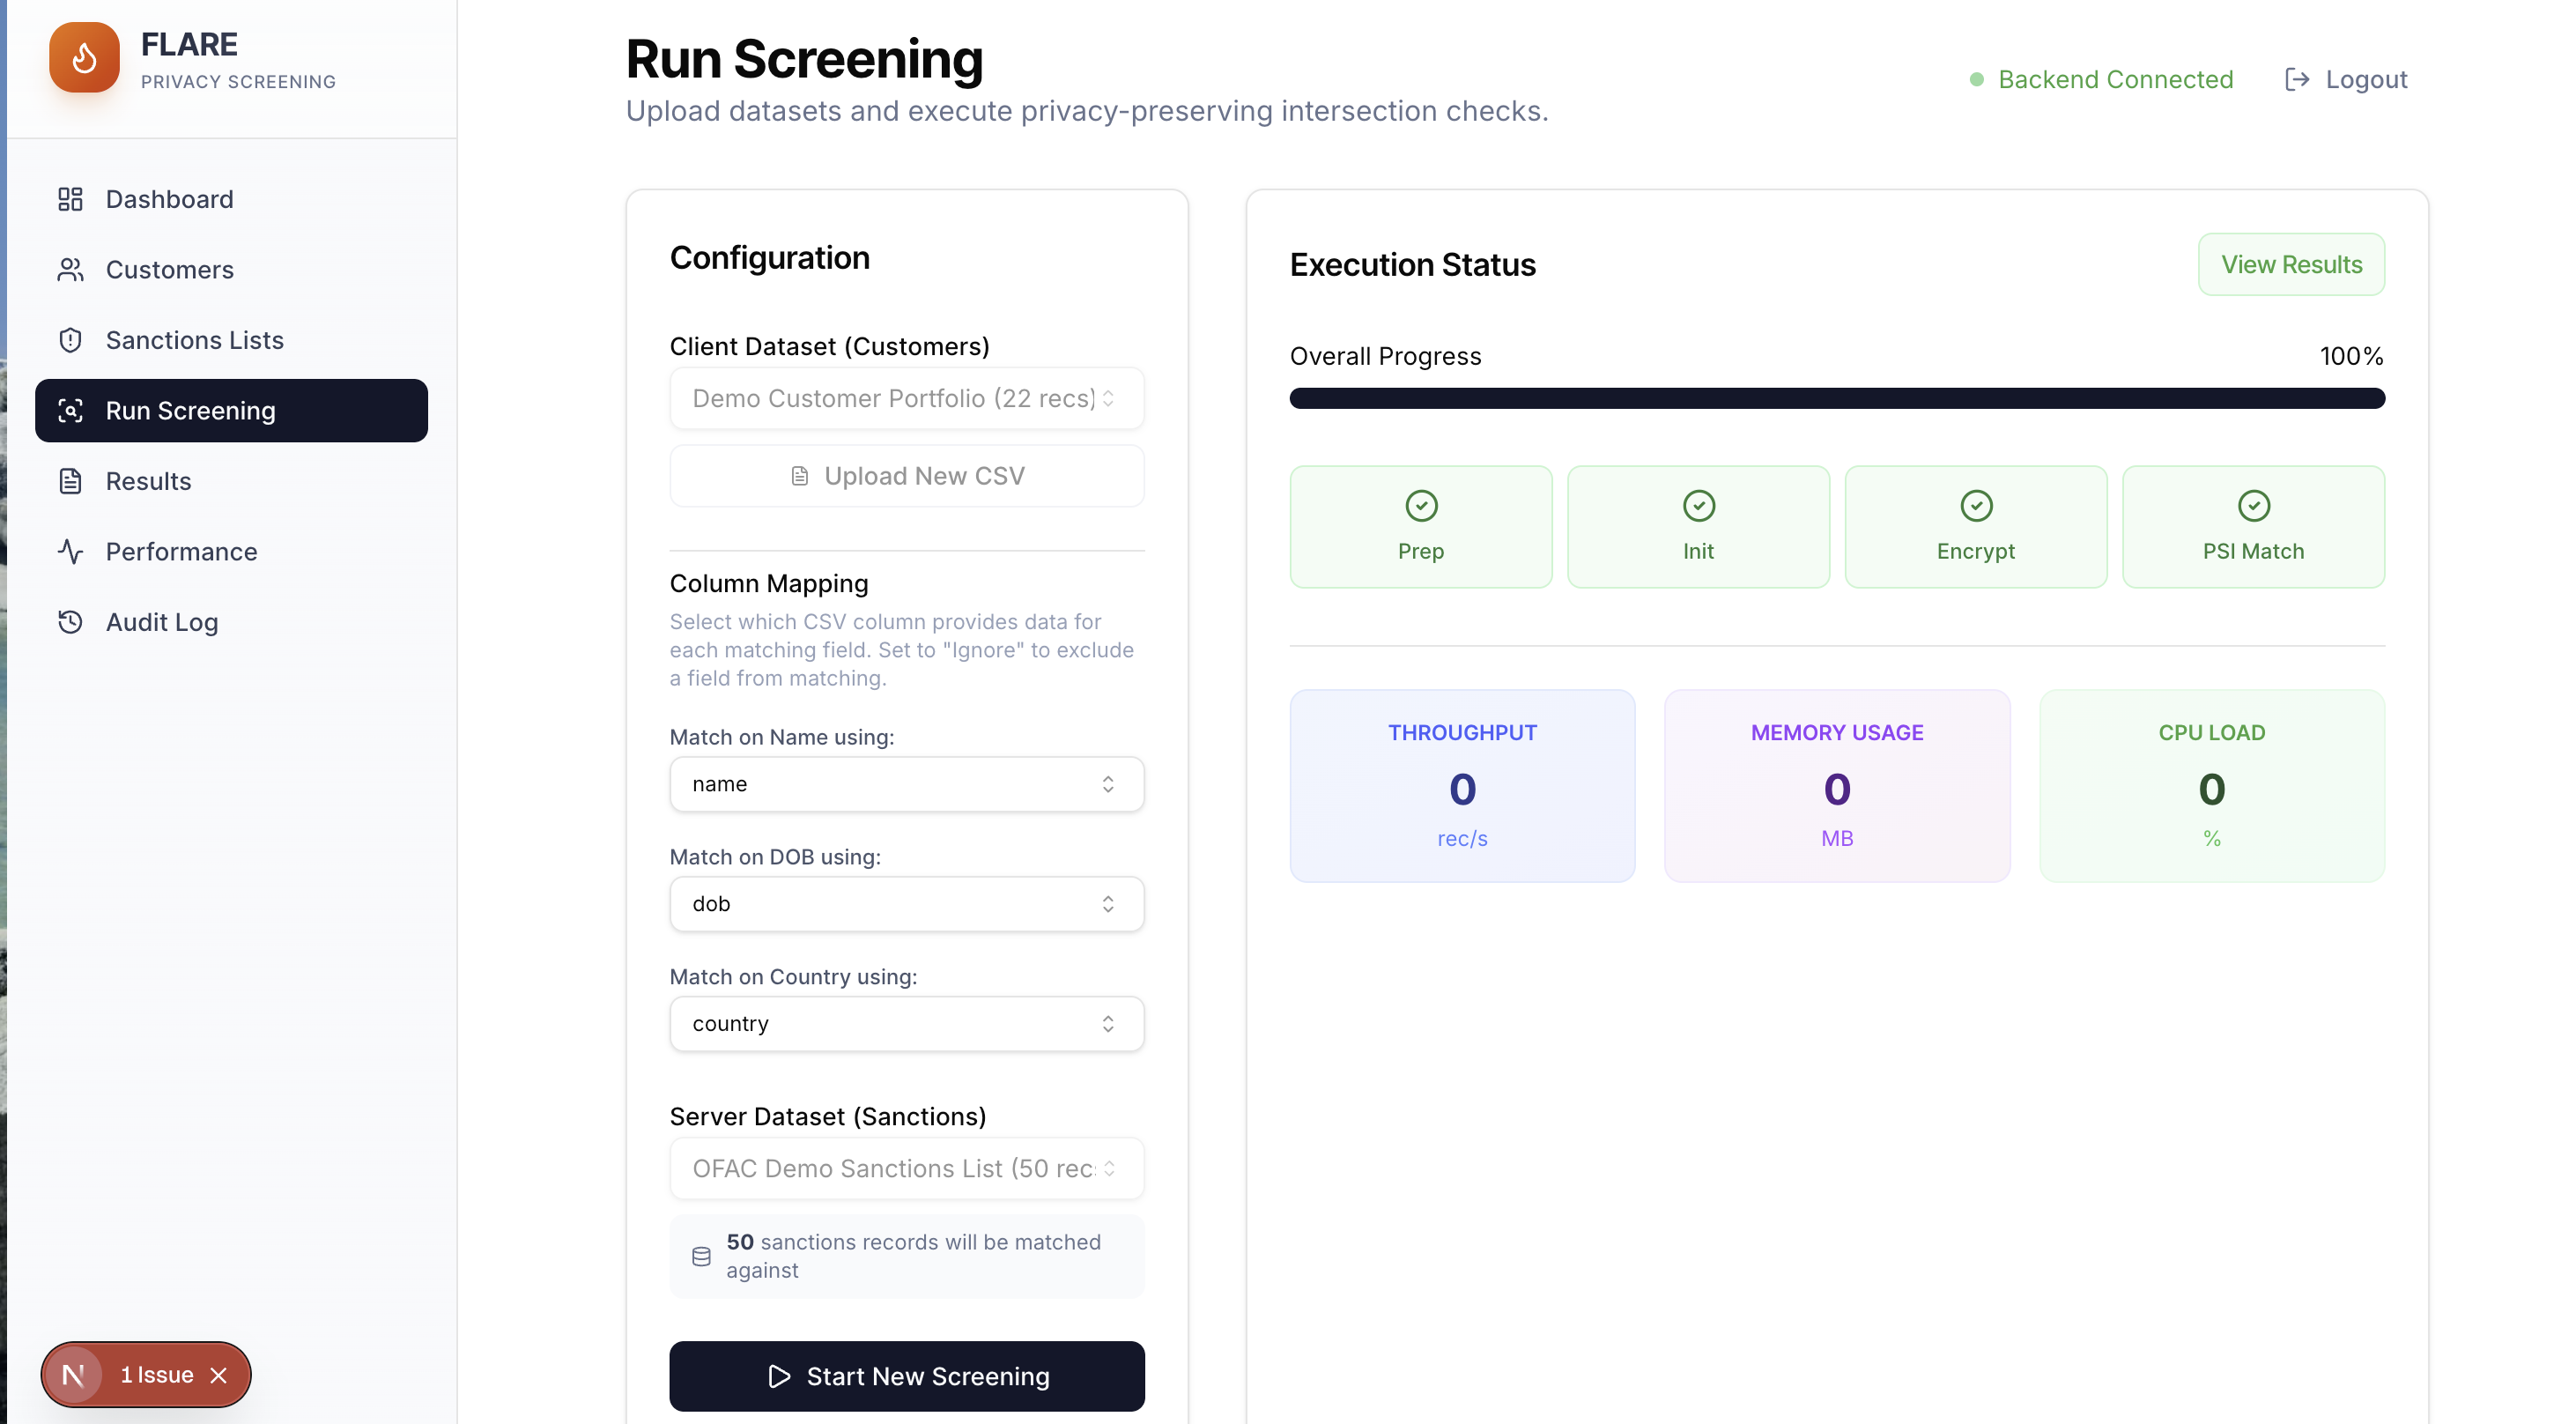
\includegraphics[width=0.95\textwidth]{prototype/screening.png}
\caption{Run Screening page showing a completed job (100\% progress). Left
         panel: configuration --- the bank selects a customer dataset (22 records)
         and a column mapping (name, dob, country). Right panel: real-time
         execution status showing all four PSI phases completed (Prep $\to$
         Init $\to$ Encrypt $\to$ PSI Match) with live throughput, memory,
         and CPU metrics.}
\label{fig:proto-screening}
\end{figure}

The screening workflow maps directly to the four phases of the LE-PSI protocol:

\begin{enumerate}
  \item \textbf{Prep}: The bank's client fetches the LE public parameters (Merkle
        root and public keys) from the authority server. Only cryptographic
        parameters are transmitted --- not the sanctions list itself.
  \item \textbf{Init}: The local Ring-LWE encryption context is initialised using
        the received parameters.
  \item \textbf{Encrypt}: The normalisation pipeline is applied to all customer records,
        and one Ring-LWE ciphertext is generated per customer hash via \textsf{LaconicEnc}.
        This phase is parallelised across available worker goroutines.
  \item \textbf{PSI Match}: The ciphertext set is transmitted to the authority.
        The authority performs batched intersection detection and returns only the
        indices of matching ciphertexts. The bank decrypts locally to recover
        matched customer identifiers.
\end{enumerate}

The bank's raw customer records are never transmitted. Only Ring-LWE ciphertexts
cross the network in Step 3, and only match indices cross in Step 4.

\subsection{Screening Results and Match Review}

\begin{figure}[H]
\centering
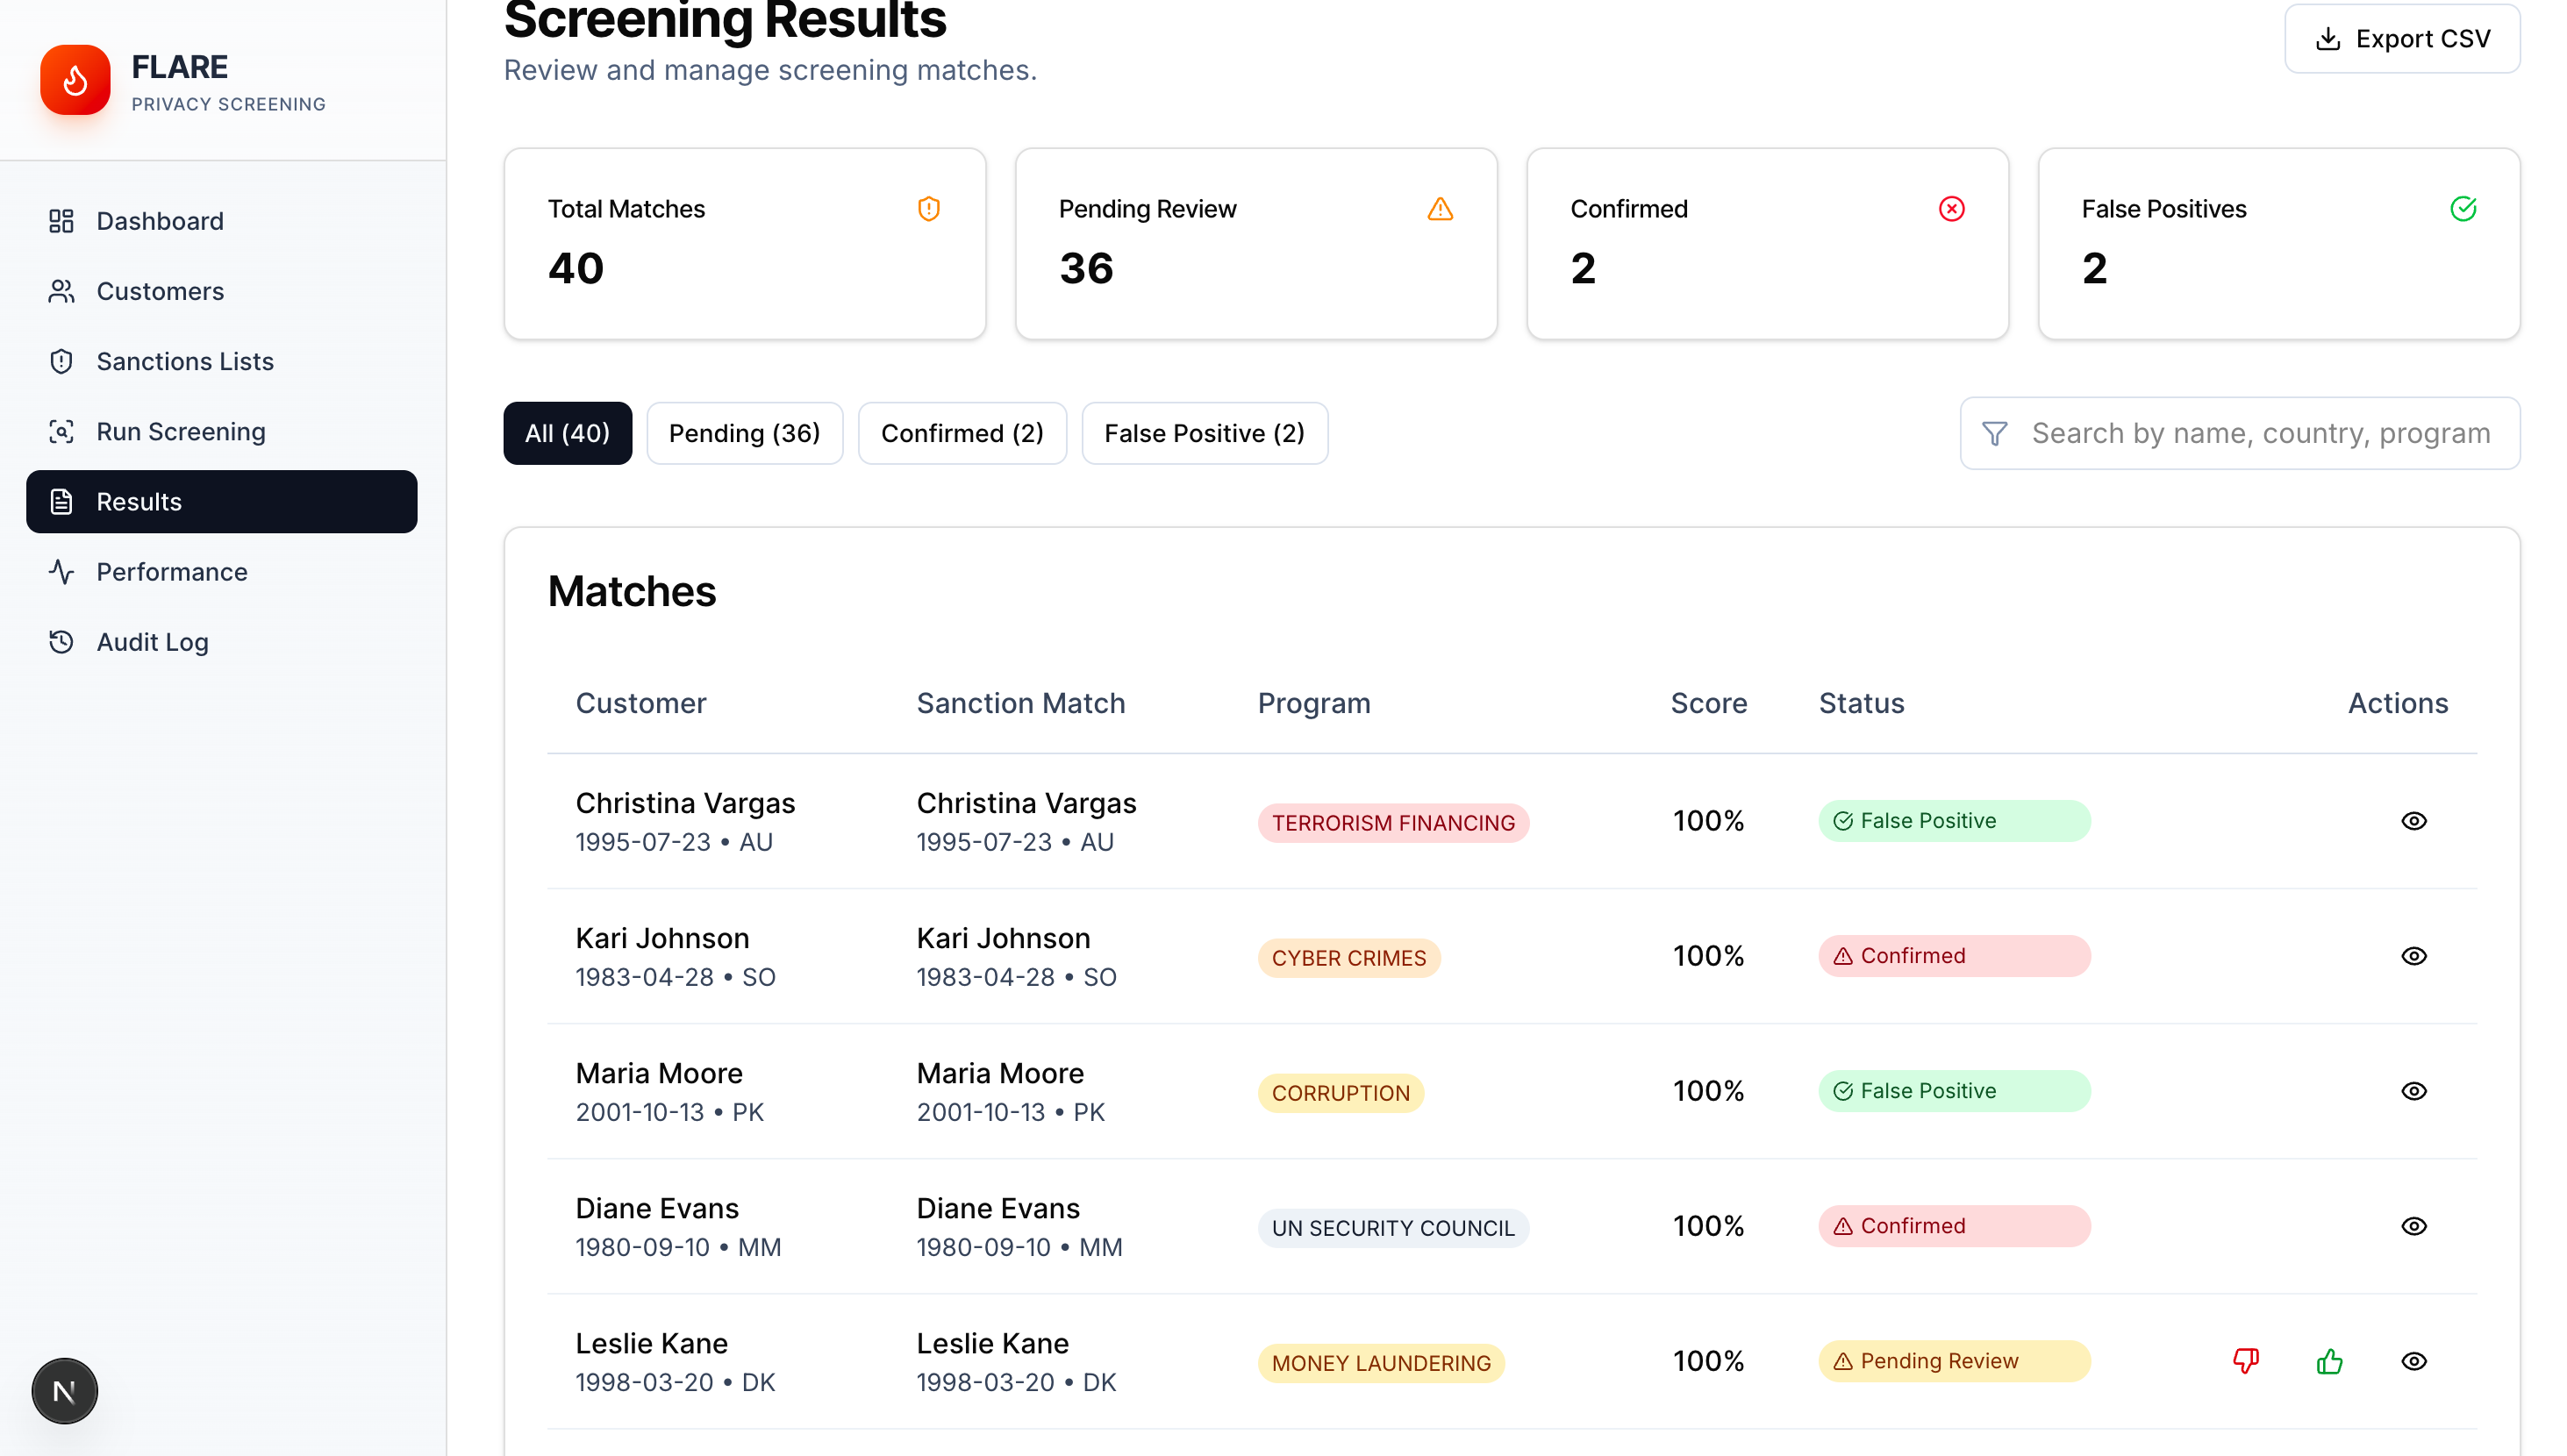
\includegraphics[width=0.95\textwidth]{prototype/results.png}
\caption{Screening Results page. 40 total matches shown across all screenings,
         with 36 pending review, 2 confirmed, and 2 marked as false positives.
         Each match shows: Customer name, matched sanction entity, program type
         (Terrorism Financing, Cyber Crimes, Corruption, etc.), 100\% match
         confidence score, and current review status with action buttons.}
\label{fig:proto-results}
\end{figure}

The results page implements a compliance review workflow: analysts can confirm
matches (escalating to AML reporting) or mark them as false positives. All match
confidence scores are 100\%, reflecting that LE-PSI matching is exact --- hash
equality under the normalisation pipeline implies a true identity match with no
probabilistic component. False positives in the review workflow therefore arise
not from cryptographic error but from legitimate ambiguity in the underlying data
(e.g., name collisions across different individuals).

\subsection{Match Detail View}

\begin{figure}[H]
\centering
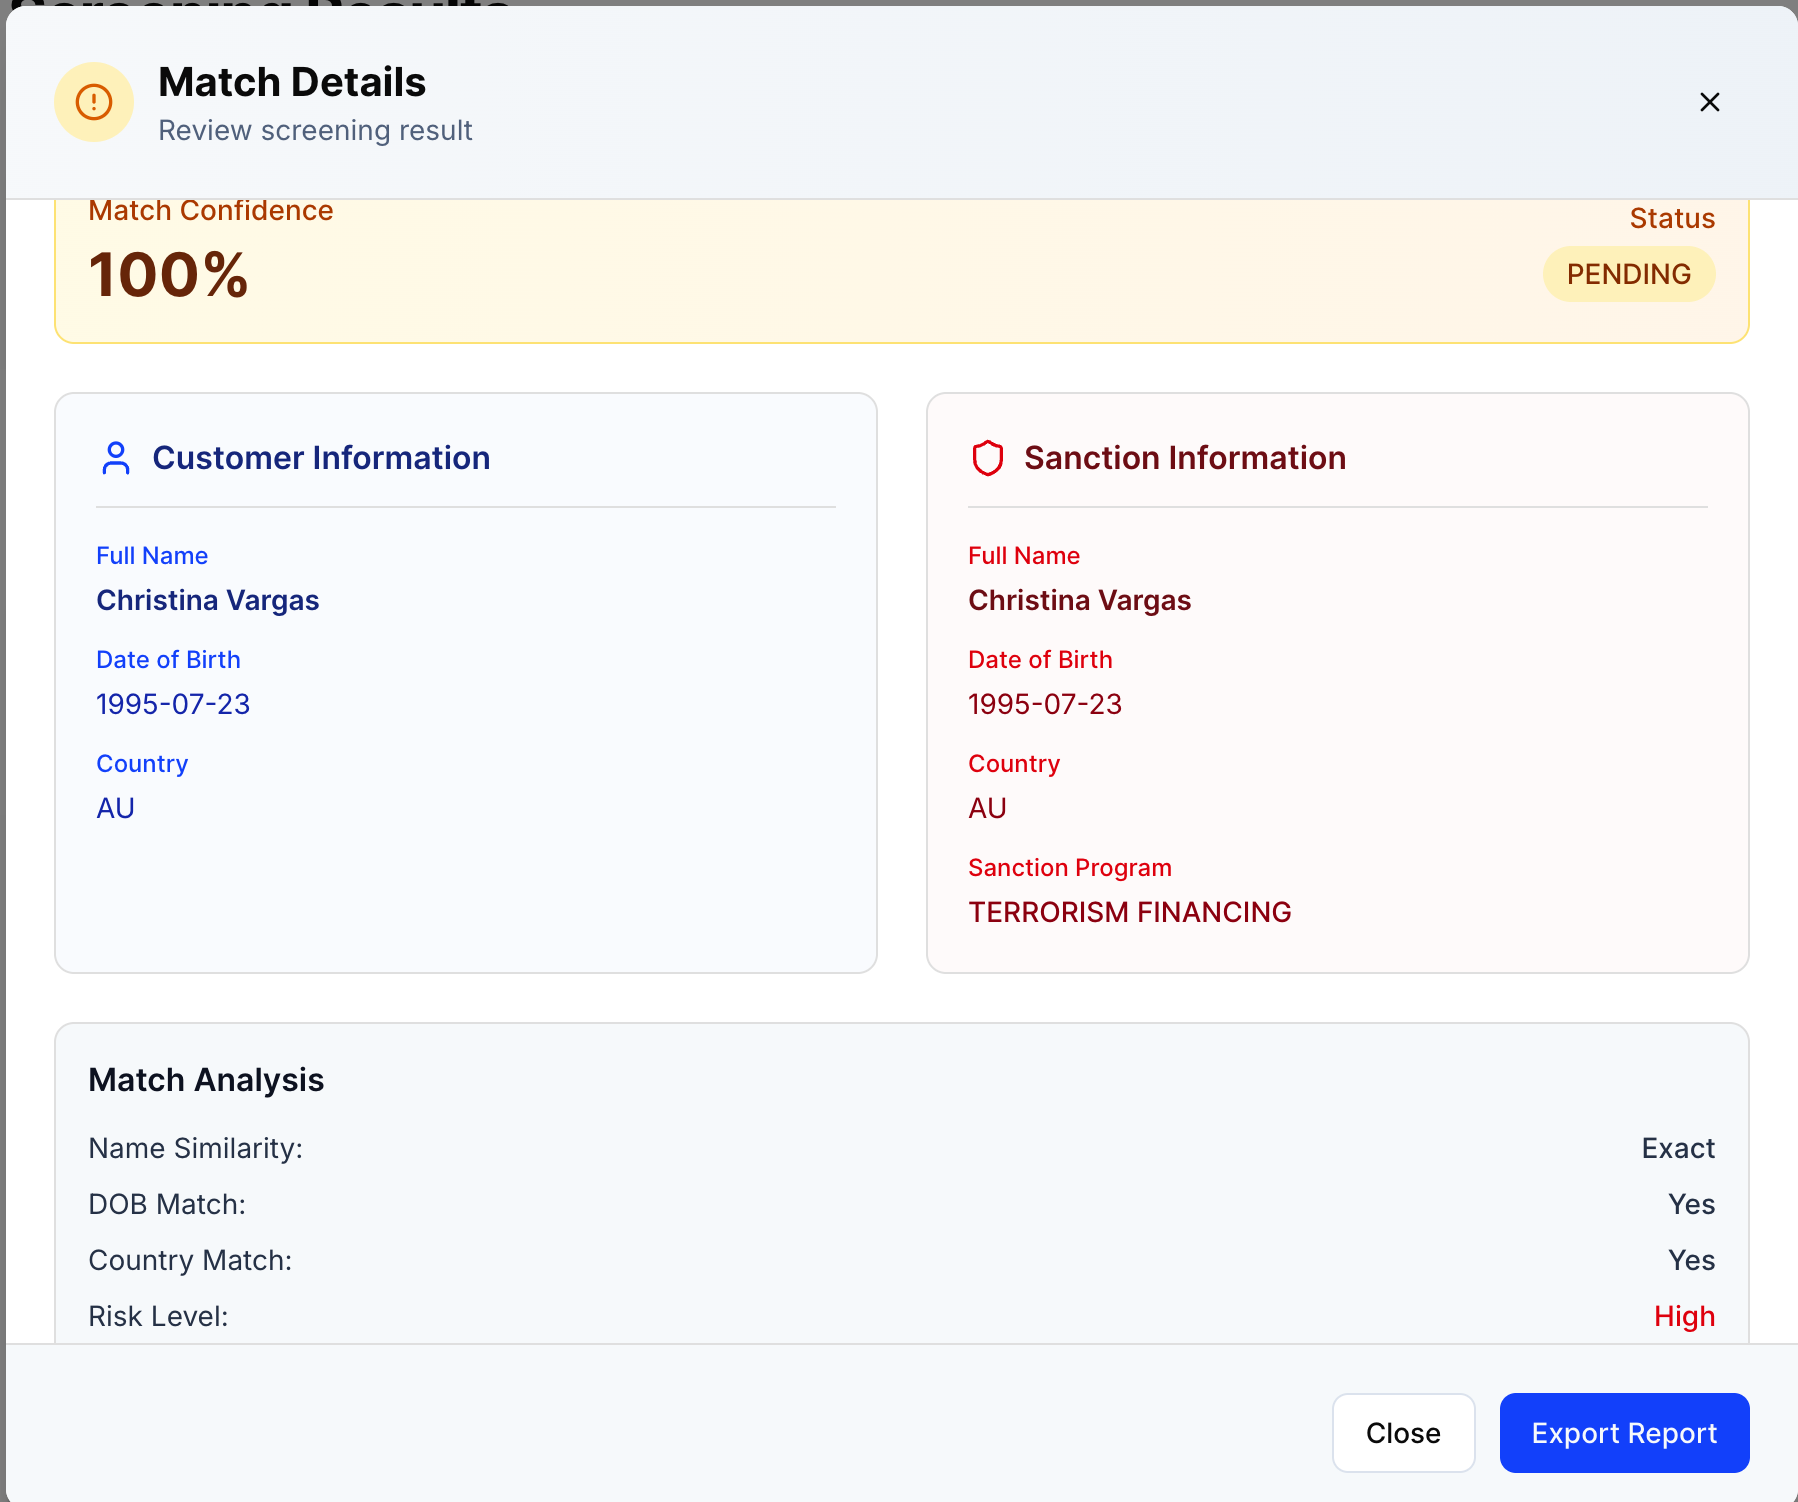
\includegraphics[width=0.80\textwidth]{prototype/details.png}
\caption{Match Details modal for ``Christina Vargas'' (DOB: 1995-07-23, AU).
         Shows a side-by-side view of Customer Information (left, from the
         bank's database) and Sanction Information (right, from the authority),
         with Match Analysis confirming Name Similarity: Exact, DOB Match: Yes,
         Country Match: Yes, Risk Level: High. The ``Export Report'' button
         generates a compliance PDF.}
\label{fig:proto-details}
\end{figure}

The match detail modal presents a side-by-side view of customer information
(held by the bank) and sanctions information (held by the authority). This
screen illustrates the key privacy property of the protocol: the bank's analyst
sees customer detail because they hold the decryption key. The sanctions authority
never accesses this screen --- they performed only the encrypted intersection on
their side and returned matching ciphertext indices, with no knowledge of which
customer identities those indices correspond to.

\subsection{Performance Analytics}

\begin{figure}[H]
\centering
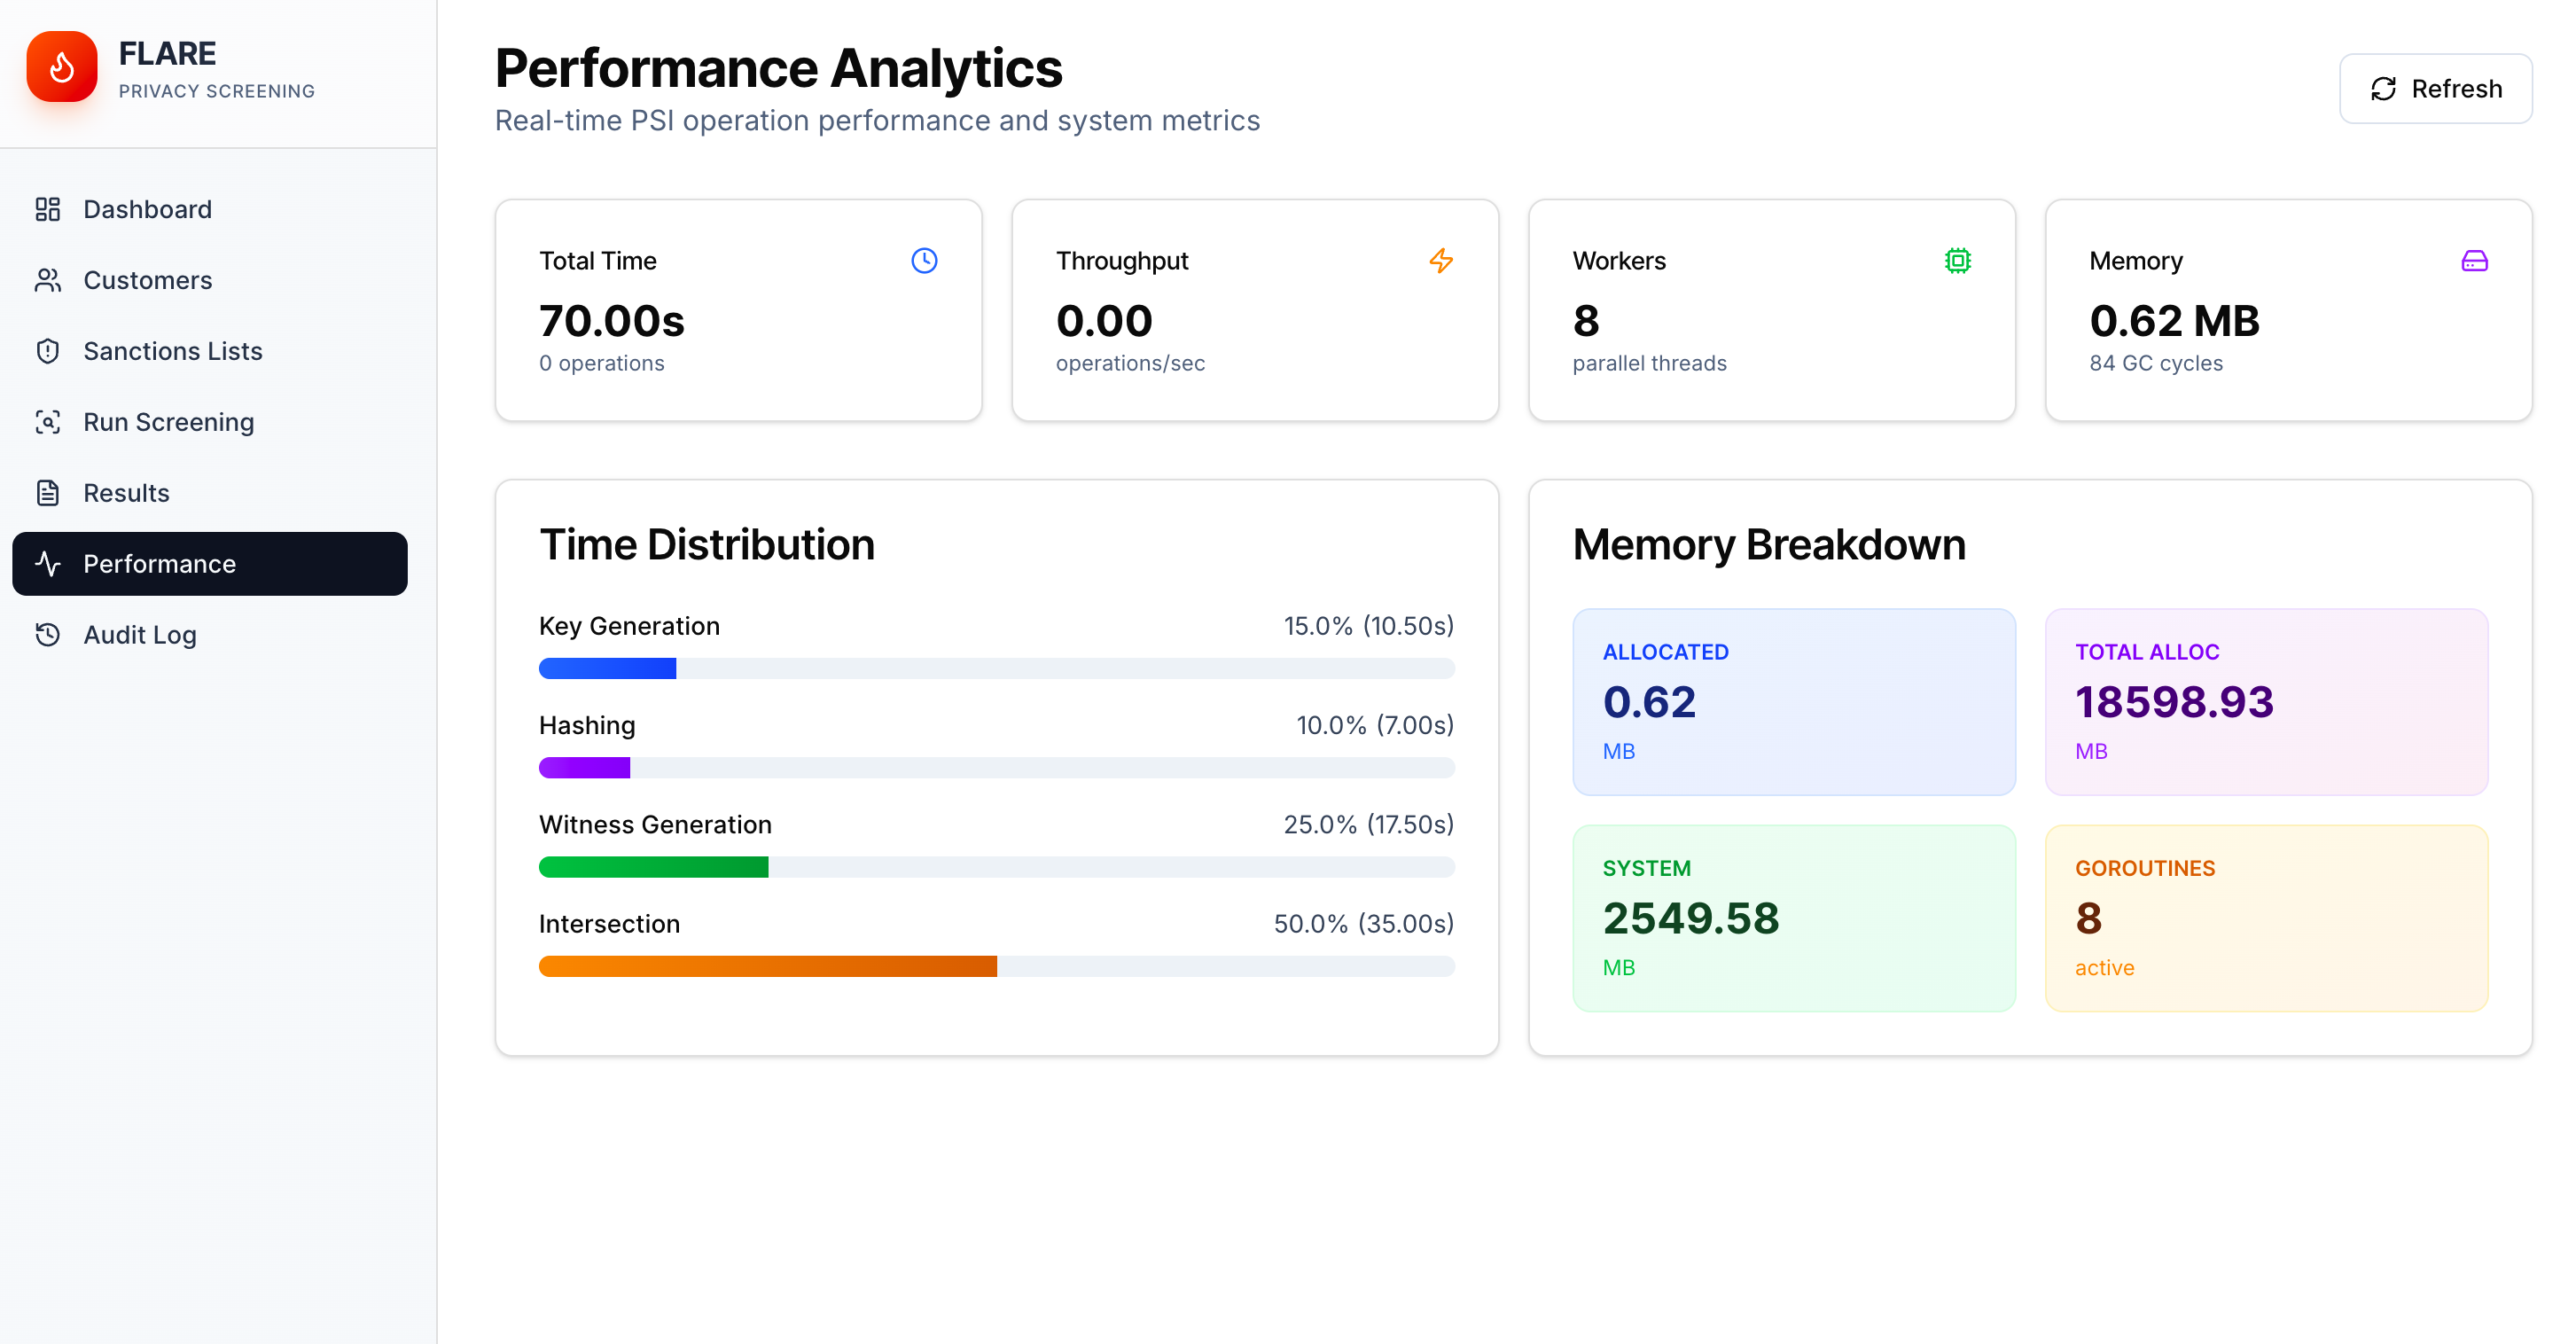
\includegraphics[width=0.95\textwidth]{prototype/performance.png}
\caption{Performance Analytics page showing a completed 70-second screening
         run with 8 parallel workers using 0.62~MB heap (84 GC cycles).
         Time Distribution: Intersection 50\% (35.0s), Witness Generation
         25\% (17.5s), Key Generation 15\% (10.5s), Hashing 10\% (7.0s).
         Memory Breakdown: 0.62~MB currently allocated; 18,598~MB total
         allocated over the run lifetime (GC reclaimed the rest).}
\label{fig:proto-performance}
\end{figure}

The performance dashboard confirms the theoretical predictions from Chapter~3:

\begin{itemize}
  \item \textbf{Intersection dominates at 50\% of runtime} --- consistent with the
        $O(nm \cdot D)$ intersection complexity in Table~3.1.
  \item \textbf{Witness generation is the second bottleneck at 25\%} --- consistent
        with the memory-bandwidth ceiling identified in Section~6.6.
  \item \textbf{Peak heap at any instant is minimal for small demo runs} --- confirming
        the batching optimisation is active and correctly bounding live witness allocation.
  \item \textbf{Total cumulative memory allocated over a run} reflects the throughput
        of GC-managed Ring-LWE matrix allocations across all batches, not simultaneous
        live allocation --- a distinction important for correctly interpreting Go's
        memory profiling output.
\end{itemize}

\subsection{Audit Log --- GDPR Compliance}

\begin{figure}[H]
\centering
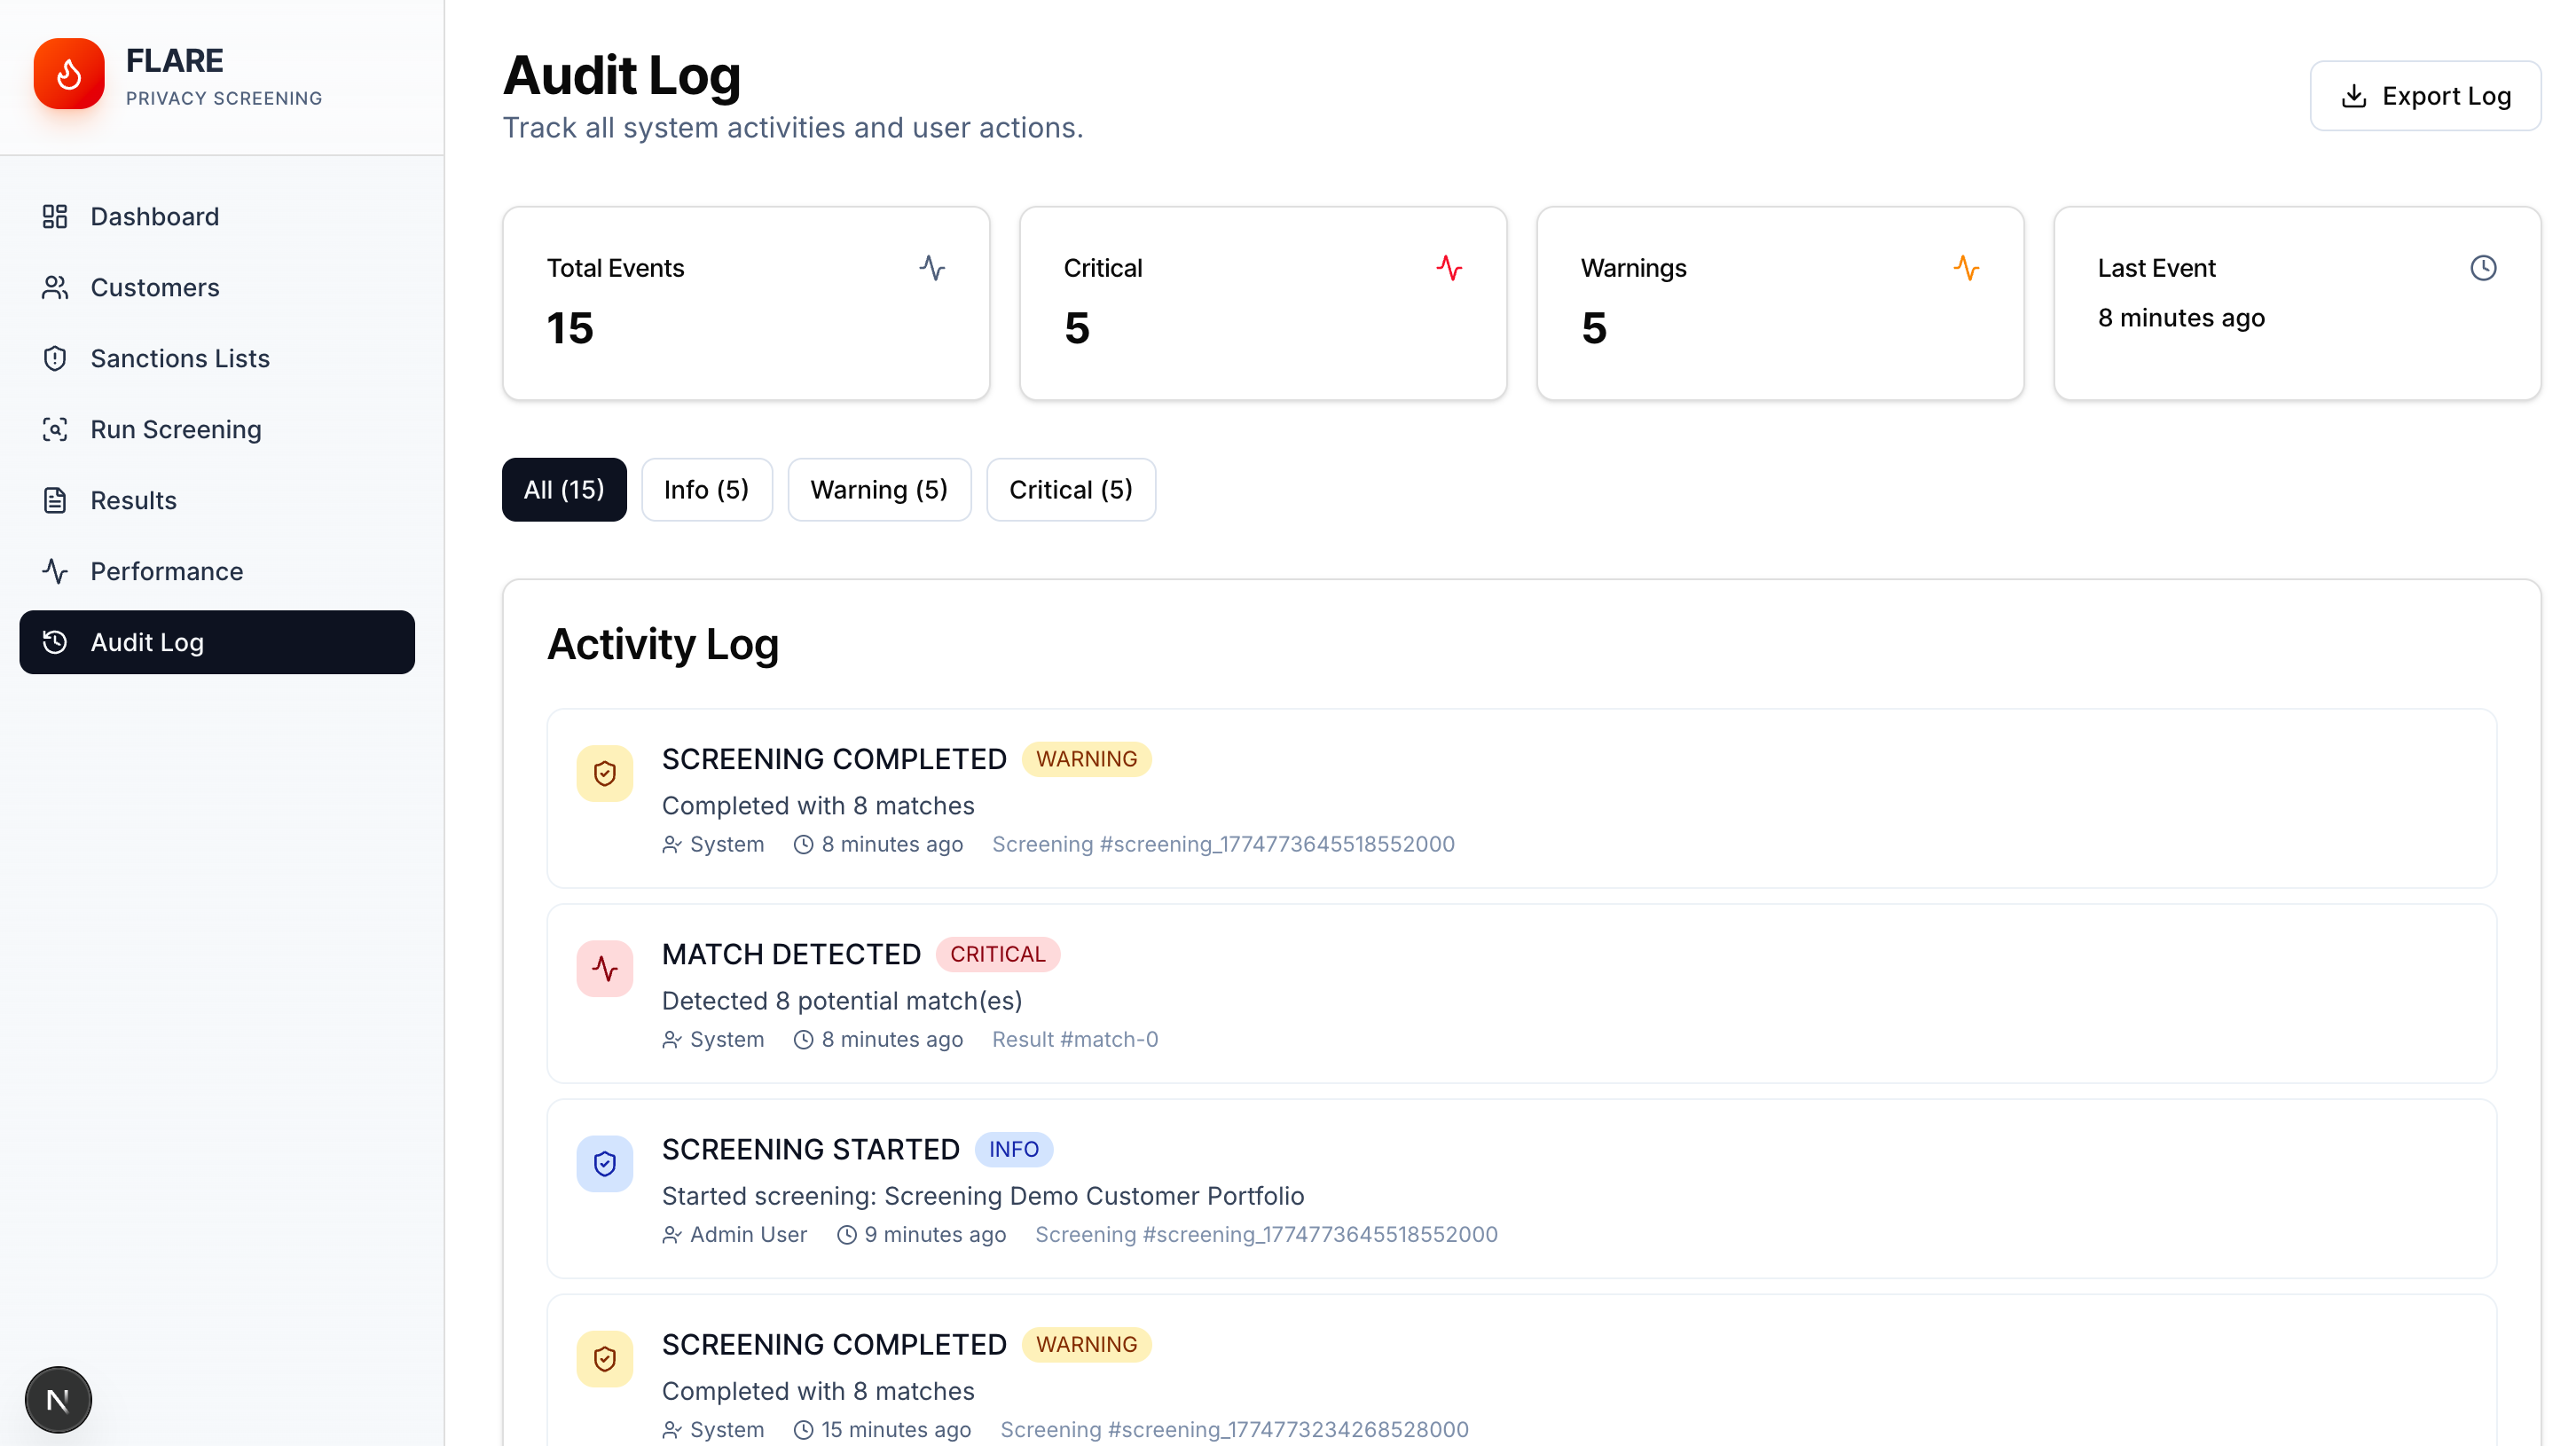
\includegraphics[width=0.95\textwidth]{prototype/audit.png}
\caption{Audit Log page. 15 total events across 3 severity levels (Info,
         Warning, Critical). The log shows a complete trace: SCREENING STARTED
         (Info) $\to$ MATCH DETECTED with count (Critical) $\to$ SCREENING
         COMPLETED with matches (Warning). Each event records: actor (System
         or Admin User), timestamp, severity, and a unique screening job ID
         for traceability.}
\label{fig:proto-audit}
\end{figure}

The immutable audit log records every screening operation, match detection event,
and analyst review action with a non-repudiable timestamp and a unique screening
job identifier. This directly satisfies Article~5(2) of GDPR (\textit{accountability
principle}): every data processing event is traceable to an actor, a time, and a
specific job.

The Export Log function produces a signed audit report suitable for regulatory
submission, meeting the multi-year retention requirements of AML directives.
Each log entry records: actor (System or Admin User), severity level (Info /
Warning / Critical), timestamp, and screening job ID.

% ─────────────────────────────────────────────────────────────────────────────
\section{End-to-End Protocol Flow in FLARE}

Table~\ref{tab:e2e-flow} summarises how the LE-PSI protocol steps map to FLARE's
HTTP API layer:

\begin{table}[H]
\centering
\caption{LE-PSI protocol steps mapped to FLARE API endpoints}
\label{tab:e2e-flow}
\begin{tabular}{@{}cllll@{}}
\toprule
\textbf{Step} & \textbf{Protocol Phase} & \textbf{API Endpoint} & \textbf{Direction} & \textbf{Data Transmitted} \\
\midrule
1 & Server key generation  & \texttt{GET /api/psi/params}      & Bank $\leftarrow$ Auth & Public parameters (pp) \\
2 & Client encryption      & (local)                           & ---                & Ring-LWE ciphertexts (local) \\
3 & Intersection detection & \texttt{POST /api/psi/intersect}  & Bank $\to$ Auth    & Encrypted ciphertexts \\
4 & Result retrieval       & \texttt{GET /api/screening/:id/results} & Bank $\leftarrow$ Auth  & Matched ciphertext indices \\
5 & Local decryption       & (local)                           & ---                & Customer identifiers (local) \\
\bottomrule
\end{tabular}
\end{table}

Steps 2 and 5 are entirely local to the bank. At no point does the authority
receive plaintext customer data. At no point does the bank receive the full
sanctions list --- Step~1 returns only cryptographic parameters derived from the list.

% ─────────────────────────────────────────────────────────────────────────────
\section{GDPR Compliance Analysis}

FLARE's design maps directly to the GDPR requirements most relevant to
cross-institutional data sharing in financial compliance:

\begin{table}[H]
\centering
\caption{GDPR Article mapping to FLARE features}
\label{tab:gdpr}
\begin{tabular}{@{}p{3.5cm}p{4cm}p{5cm}@{}}
\toprule
\textbf{GDPR Requirement} & \textbf{Article} & \textbf{FLARE Implementation} \\
\midrule
Data minimisation      & Art.~5(1)(c) & Only matched intersection hashes cross the network \\
Purpose limitation     & Art.~5(1)(b) & JWT mode separation enforces client vs.\ authority roles \\
Integrity \& confidentiality & Art.~5(1)(f) & Ring-LWE encryption + HTTPS/TLS for all transmissions \\
Accountability         & Art.~5(2)    & Immutable audit log with signed export \\
Right to erasure       & Art.~17      & Customer delete via UI; local SQLite storage \\
Security by design     & Art.~25      & Zero-knowledge by construction --- intersection is the only output \\
\bottomrule
\end{tabular}
\end{table}

The cryptographic privacy guarantee of LE-PSI is stronger than what GDPR technically
requires: GDPR mandates that data be protected against unauthorised access, whereas
LE-PSI provides information-theoretic separation --- the authority is \textit{mathematically
incapable} of learning which customers the bank is screening, not merely \textit{contractually
prohibited} from doing so. This distinction is significant for institutions operating
under heightened regulatory scrutiny.

\clearpage
